\chapter{Evaluation}\label{chapter:eval}

In this chapter we summarize the key results we reached by running SymNet on
various models generated by our tool, \TOOL.  It is divided in two sections.
In the first one we argue that the models we build capture the packet
processing logic behind netfilter.  In the second one we use models built from
synthetic rules to evaluate the quality of our code generation approach
discussed in previous chapters.


\section{Acceptance tests}

Acceptance tests help answer the question \emph{"Does our model reflect the
semantics of netfilter, the real system?"}  Certainly we would rather not
introduce inconsistencies in a software system that is supposed to find bugs in
another one. In some formal verification systems the \emph{model - real system}
equivalence is enforced by construction.  However, this is not true in SymNet
for reasons described in \labelindexref{Section}{sec:symnet-sefl}, and, thus,
we need to run hand-crafted tests to confirm our expectations.

Driven by this insight from the very beginning, we have performed extensive
unit testing, focusing on specific components and/or behaviours, as well as
integration testing, when linking them together.  Our testing suite contains
more than \textbf{130 total tests} and achieves over \textbf{91\% code
coverage}~\cite{github-repo}.  This means that we have generated models that
cover most of our model generation corner cases.  However, this should not be
confused with \emph{generated code} coverage, which depends on input packet,
input port, as well as the interaction with the network as a whole, considering
that some of the networks elements that we model are stateful.

In the following paragraphs we show a small subset of the scenarios that we
tested against.

\paragraph{Simple NAT policy.}
We start with a very simple example to give an intuition of how these tests are
performed by including the Scala code too.

\labelindexref{Listing}{lst:unreachable-rule} shows the entire test.  Between
\textbf{lines 2-7} the nat/POSTROUTING chain is set up with two rules: one to
match an entire private network (\lstinline{-s 192.168.1.0/24}) and the other
one to only match a host in the  same network (\lstinline{-s 192.168.1.100}).
Between \textbf{lines 8-13} we run symbolic execution injecting a packet with
the source IP set to \lstinline{192.168.1.100} (line 12), starting from this
chain's input port (lines 10-11).  Between \textbf{lines 14-19} we define the
\emph{rewrite constrain} that we expect to take place.  Finally, at line 22 we
\textbf{express the policy} using the custom Scala matcher,
\emph{containConstrain} that looks up the given constrain in the list of
successful paths output by symbolic execution.

\begin{listing}[H]
  \caption{An example of a NAT misconfiguration taken from a \emph{Local Area
  Networks} lecture quick.  Notice that Scala already makes policy
  specification easy to understand owing to its relaxed syntax rules.}
  \label{lst:unreachable-rule}
  \sourcecode{scala}{src/code/simple-nat.scala}
\end{listing}

This example is intended to show how a network administrator would express
policies and catch inconsistencies.  Indeed, this test fails because the
specified host IP matches the first rule in the table.  In fact, the second
rule will never be matched, indicating a misconfiguration which would hopefully
be found as a result of the policy failing.

\paragraph{NAT-ed connections.}
To take our previous SNAT configuration from a toy example that is intended to
give a glimpse at how simple policies can be expressed in code to an
end-to-end one, we use a network topology as shown in
\labelindexref{Figure}{fig:source-nating}.

\begin{figure}[h]
  \centering
  \captionsetup{justification=centering}
  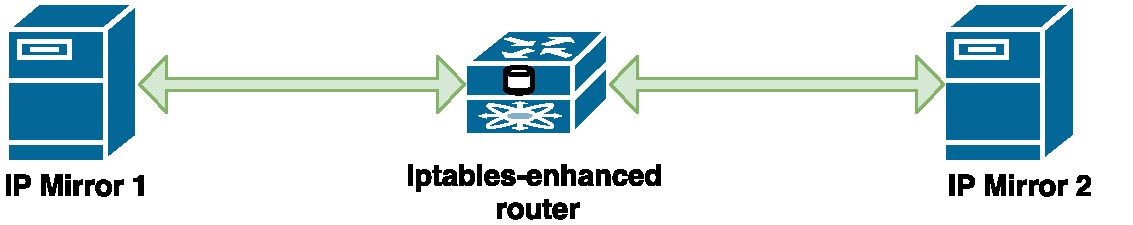
\includegraphics[scale=0.5]{src/img/source-nating}
  \caption{Generic network configuration used to test various stateful
  functions.}
  \label{fig:source-nating}
\end{figure}

The \textbf{IP mirror} component is used to model reply packets.  Thus, by
connecting two of them through an intermediate device that is our
iptables-enhanced router, we obtain bi-directional communication between them.
This is in fact a pattern we often use when testing any kind of stateful
configuration.  It is not tied to NAT-ing in any way.

How do we specialize it for NAT testing?  Besides the rules that define our
model, the specific scenarios that we test are controlled by input packets and
input ports.  For instance:
\begin{itemize}
  \item To test that SNAT rules are \textbf{correctly applied}, we inject an
    initial packet that matches the rule we are interested in on the output
    port of \emph{IP mirror 1} and check if a packet with the rewritten source
    IP reaches the input port of \emph{IP mirror 2}.
  \item To test that \textbf{reverse} SNAT rules are correctly applied, we add
    one more policy rule to the previous example: a packet with the reverse
    source/destination IPs should reach the input port of \emph{IP mirror 1}.
  \item To test that the nat/POSTROUTING chain is traversed \textbf{only once}
    for a SNAT-ed connection, we add the following policy rule: the input port
    of this particular chain is traversed only once.  The special logic for
    skipping it otherwise is subjected to test here.
  \item To test that the same rule does not apply if the connection is
    initiated from the \textbf{opposite direction} (SNAT rules use source IP
    matches, in general), we inject a packet on the output port of \emph{IP
    mirror 2} and check that a packet with the rewritten source IP \textbf{does
    not} reach the input port of \emph{IP mirror 1}.
  \item To make the previous scenario work, we change our model by adding a
    DNAT rule in the nat/PREROUTING chain.  We make sure that all previous
    policies are still valid.
\end{itemize}

This is a non-exhaustive list but gives a good idea of the challenges behind
Network Address Translation testing.

\paragraph{Connection state switch.}
Another key feature that has been thoroughly tested is the transition between
connection states.

The network model we built to test it is shown in
\labelindexref{Figure}{fig:state-switch}.  It consists of our regular
iptables-enabled device (left) and an IP mirror element that is used to
generate reply packets, as previously described (right).  We simulate traffic
from our device to the server by injecting a concrete packet on the output port
of the local process component.  As discussed at the end of
\labelindexref{Chapter}{chapter:model}, we expose this port as part of the
interface of our model precisely for this reason
(\labelindexref{Figure}{fig:local-process-out}).

A new metadata field is stored for each packet flow to track its connection
state, intuitively called \textbf{ctstate}.  The first time a packet belonging
to a connection is seen, its \emph{ctstate} is set to \NEW (transition
\textbf{1 -> 2}).  Once a packet in the \textbf{reverse} direction is
processed, the state becomes \ESTABLISHED (transition \textbf{3 -> 4}).  Our
policy in this case can be stated such as: \emph{there must be a packet flow
that reaches the local process and its ctstate field is ESTABLISHED}.

\begin{figure}[h]
  \centering
  \captionsetup{justification=centering}
  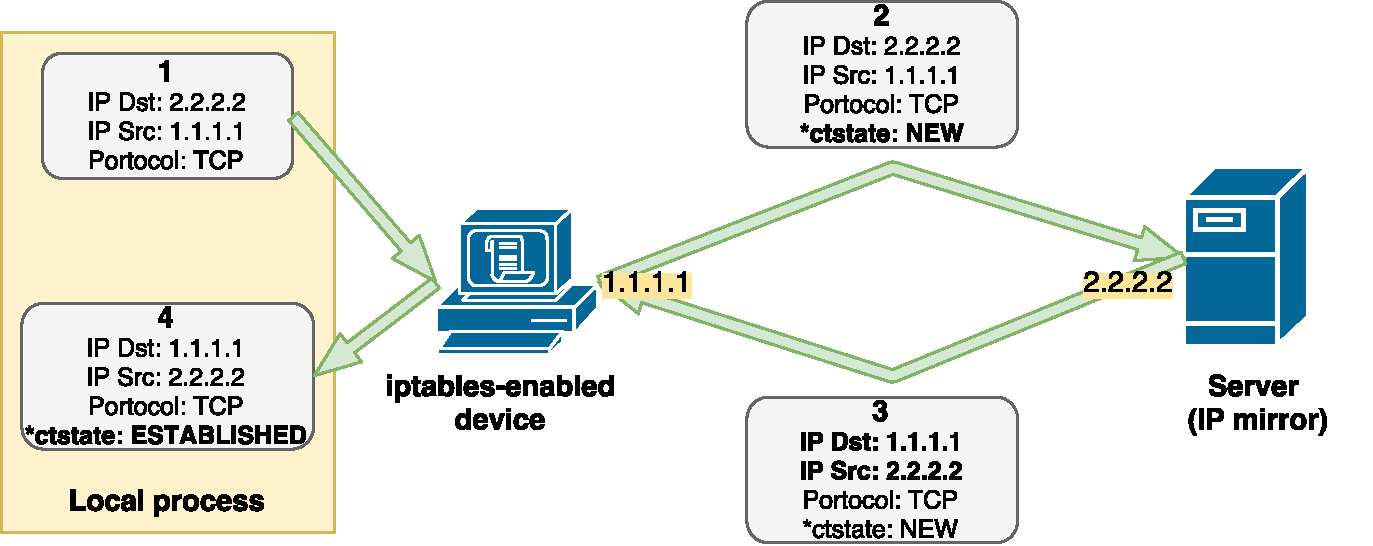
\includegraphics[scale=0.5]{src/img/state-switch}
  \caption[Network model built to test connection tracking.]{Network model
  built to test connection tracking. Fields in bold font are the ones modified
  in the last step.}
  \label{fig:state-switch}
\end{figure}

\paragraph{Untracked connection.}
As a follow-up scenario for the previous one, we also ensured that marking
certain traffic as \UNTRACKED in the \emph{raw} table leads to no state
transitions.

\bigskip

An alternative approach to bypassing the \emph{model - real system} equivalence
problem that we have yet to experiment with is \emph{black-box testing}.  It
requires establishing a(n) (usually large) list of input packets and injecting
them both in the real system and in its model constructed with \TOOL.  Then,
monitor output packets in the real iptables-enabled device and try to match
them against the exhaustive list of (symbolic) packet flows output by SymNet.
If for some input packet there is no symbolic flow that matches the observed
output packet, the equivalence is denied.  The inverse is obviously not
necessarily true, but it increases our \emph{belief} that the implementation is
correct.


\section{Performance tests}


Things to say:
* tests performed:
1. many rules, on a single filter table;
2. many IPTRouters in line.
* overall results
* tables/graphs

\bigskip

Besides these script-generated configurations, we have also run SymNet on a
model of a Neutron L3 agent\footnote{It is essentially a router that uses the
Linux IP stack and iptables in an isolated \emph{network namespace}.  This in
turn is the Linux terminology for the \emph{Virtual Routing and Forwarding}
(VRF)\abbrev{VRF}{Virtual Routing and Forwarding} concept that takes the idea
of Virtual Local Area Networks (VLANs)\abbrev{VLAN}{Virtual Local Area Network}
from the L2 switching world to the L3 world.} from a real OpenStack deployment.
Its complete iptables dump is included in
\labelindexref{Appendix}{app:qrouter}.

Exploring all possible execution paths by injecting a pure symbolic packet on
one of its input ports takes around \textbf{25s} and \textbf{6GB} of RAM.  This
generates 1345 packet flows.  Only 74 of them are successful.  Out of all
failed ones only 6 are explicitly dropped.  The remaining ones are packets
caused by internal logic of our model that cannot be materialized.  Since there
are only two rules that DROP packets, it becomes manageable to inspect those
packets by hand.  Moreover, if we constrain just the destination IP address of
the injected packet to a concrete value, symbolic execution time drops to
\textbf{5s}.  This shows the importance of having a policy drive symbolic
execution rather than exploring all possible execution outcomes.
